%%%%%%%%%%%%%%%%%%%%%%%%%%%%%%%%%%%%%%%%%%%%%%%%
%% Compile the master file!
%% 		Slides: Antonio Machicao y Priemer
%% 		Course: Wissenschaftliches Arbeiten
%%%%%%%%%%%%%%%%%%%%%%%%%%%%%%%%%%%%%%%%%%%%%%%%


%%%%%%%%%%%%%%%%%%%%%%%%%%%%%%%%%%%%%%%%%%%%%%%%%%%%
%%%             Metadata                         
%%%%%%%%%%%%%%%%%%%%%%%%%%%%%%%%%%%%%%%%%%%%%%%%%%%%  

\title{
	\LaTeX\ for Linguists
}

\subtitle{\LaTeX\ 4: Bibliography}

\author[aMyP]{
	{\small Sebastian Nordhoff \& Antonio Machicao y Priemer}
	\\
	{\footnotesize \url{www.linguistik.hu-berlin.de/staff/amyp}}
	%	\\
	%	{\footnotesize \href{mailto:mapriema@hu-berlin.de}{mapriema@hu-berlin.de}}
}

\institute{LOT 2019, Amsterdam}

%\date{ }

%\publishers{\textbf{6. linguistischer Methodenworkshop \\ Humboldt-Universität zu Berlin}}

%\hyphenation{nobreak}


%%%%%%%%%%%%%%%%%%%%%%%%%%%%%%%%%%%%%%%%%%%%%%%%%%%%
%%%             Preamble's End                   
%%%%%%%%%%%%%%%%%%%%%%%%%%%%%%%%%%%%%%%%%%%%%%%%%%%%      


%%%%%%%%%%%%%%%%%%%%%%%%%%%%%%%%%%%
%%%%%%%%%%%%%%%%%%%%%%%%%%%%%%%%%%%    
%% Title slide 
\begin{frame}
  \HUtitle
\end{frame}


%% Contents slide
\frame{
%\begin{multicols}{2}
	\frametitle{Contents}
%	\tableofcontents[hideallsubsections]
	\tableofcontents
	%[pausesections]
%\end{multicols}
	}


%%%%%%%%%%%%%%%%%%%%%%%%%%%%%%%%%%%%
%%%%%%%%%%%%%%%%%%%%%%%%%%%%%%%%%%%%
%% Extra literature

\nocite{Freitag&MyP15a}
\nocite{Knuth1986}
\nocite{Kopka94a}
\nocite{MyP17c}
\nocite{MyP&Kerkhof16a}
	
%%%%%%%%%%%%%%%%%%%%%%%%%%%%%%%%%%%%
%%%%%%%%%%%%%%%%%%%%%%%%%%%%%%%%%%%%


%%%%%%%%%%%%%%%%%%%%%%%%%%%%%%%%%%%%%
%%%%%%%%%%%%%%%%%%%%%%%%%%%%%%%%%%%%%
%%%% Basic literature for these slides
%
%\begin{frame}
%\frametitle{Grundlage \& empfohlene Lektüre}
%
%\dots basierend auf \citet{Freitag&MyP15a} und auf \citet{MyP&Kerkhof16a}\\
%\ras \href{https://www.researchgate.net/publication/279514740_LATEX-Einfuhrung_fur_Linguisten}{LINK}
%
%
%\nocite{Kopka94a}
%
%\end{frame}


%%%%%%%%%%%%%%%%%%%%%%%%%%%%%%%%%%
%%%%%%%%%%%%%%%%%%%%%%%%%%%%%%%%%%
\section{Bibliography with Bib\TeX }
\frame{
	\frametitle{~}
%	\begin{multicols}{2}
		\tableofcontents[currentsection, hideallsubsections]
%	\end{multicols}
}
%%%%%%%%%%%%%%%%%%%%%%%%%%%%%%%%%%

\begin{frame}[fragile]
\frametitle{Bibliographieren mit BibTeX}

\begin{itemize}
	\item \LaTeX\ provides \textbf{Bib\TeX -Tool} for references and bibliographies.
%	\LaTeX\ bietet das \textbf{Bib\TeX -Tool}, um in Dokumenten \textbf{Quellen} und \textbf{Bibliographien} einfach und vor allem einheitlich handzuhaben.
	
	\item You need:
	
	\begin{enumerate}
		\item a \textbf{bibliography database} -- an ordinary text document with the ending \ltxterm{.bib}\\
		You just need to open a \ltxterm{.txt} document and change the ending to \alert{\ltxterm{.bib}}
		
		\pause
		
		\item \textbf{citation commands} in your document (similar to \lstinline|label| and \lstinline|ref|)
		
		\pause 
		
		\item a \textbf{bibliography style} (with the ending \ltxterm{.bst} -- normally provided by a package).
	\end{enumerate}
	
\end{itemize}

\end{frame}


%%%%%%%%%%%%%%%%%%%%%%%%%%%%%%%%%%
%%%%%%%%%%%%%%%%%%%%%%%%%%%%%%%%%%
\section{Bibliography database}
\frame{
\frametitle{~}
\begin{multicols}{2}
	\tableofcontents[currentsection,hideallsubsections]
\end{multicols}
}
%%%%%%%%%%%%%%%%%%%%%%%%%%%%%%%%%%

\begin{frame}[fragile]
\frametitle{Bibliography database}

\begin{itemize}
\item an ordinary text document

\item You must change the \ltxterm{.txt} to an \alert{\ltxterm{.bib}} ending.
\end{itemize}

\begin{figure}
\centering
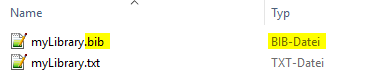
\includegraphics[width=.65\textwidth]{../../texfiles-beamer/tex-material/WissArb-latex/bib_txtDateien}
\end{figure}

\end{frame}

%%%%%%%%%%%%%%%%%%%%%%%%%%%%%%%%%%
\begin{frame}[fragile]
%\frametitle{Bibliographiedatenbank}


Entries in your database have the following syntax:

%\begin{multicols}{2}

\begin{lstlisting}
@book{Knuth1986,
author = {Knuth, Donald E.},
address = {Boston, MA},
publisher = {Addison-Wesley},
title = {The TeXbook},
year = {1986}
}
\end{lstlisting}

%\columnbreak
%
%\end{multicols}

\begin{itemize}
	\item \lstinline|@book|: type of \textbf{reference}
	\item \lstinline|{ }|: \textbf{brackets} around the complete entry \lstinline|@book{ }|\\
	and around every single information segment \lstinline|author = { }|
	
	\item \lstinline|Knuth1986|: a unique \textbf{ID} for the entry
	\item \lstinline|,|: commas as separation for the information segments
	\item \lstinline|author| \lstinline|address| etc.: type of information provided
\end{itemize}

The single information segments have always the same syntax: \lstinline|type of information = {information},|

\smallskip 

Which information depends on the \textbf{reference type} and the \textbf{bibliography style}.
\end{frame}


%%%%%%%%%%%%%%%%%%%%%%%%%%%%%%%%%%%
%\begin{frame}[fragile]
%%\frametitle{Literaturangaben}
%
%\begin{itemize}
%\item Die Datenbank können Sie \textbf{mit jedem beliebigen Texteditor} bearbeiten. 
%
%\item Verwenden Sie \ltxpack{TeXstudio} für die Bearbeitung Ihrer \ltxterm{.bib}-Datei, werden die verschiedenen Teile besonders \textbf{hervorgehoben}.
%
%
%\end{itemize}
%
%\begin{figure}
%\centering
%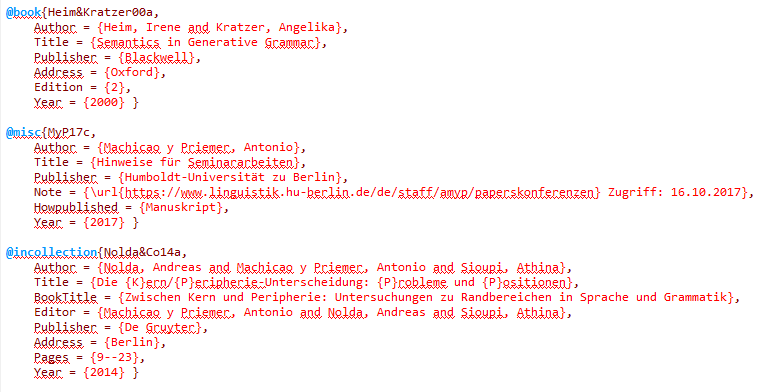
\includegraphics[width=.90\textwidth]{../../texfiles-beamer/tex-material/WissArb-latex/bibeintraege}
%\end{figure}
%
%\nocite{Heim&Kratzer00a}
%\nocite{MyP17c}
%\nocite{Nolda&Co14a}
%
%\end{frame}


%%%%%%%%%%%%%%%%%%%%%%%%%%%%%%%%%%%
%\begin{frame}[fragile]
%%\frametitle{Literaturangaben}
%
%\begin{itemize}
%
%\item Ist die Datei in \ltxpack{TeXstudio} offen, werden die IDs bei der \textbf{Autovervollständigung} angezeigt.
%\end{itemize}
%
%\begin{figure}
%\centering
%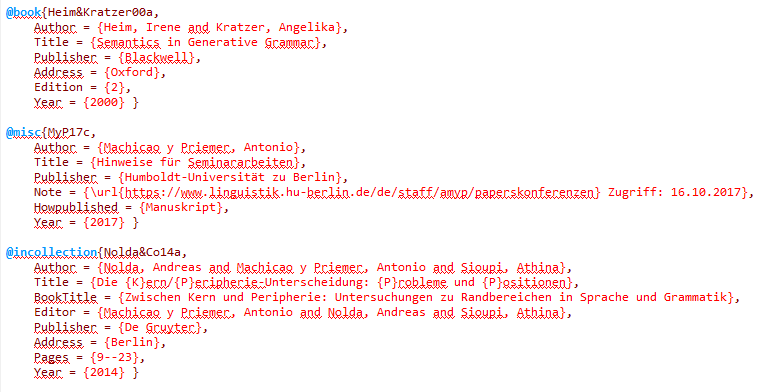
\includegraphics[width=.90\textwidth]{../../texfiles-beamer/tex-material/WissArb-latex/bibeintraege}
%\end{figure}
%
%\end{frame}


%%%%%%%%%%%%%%%%%%%%%%%%%%%%%%%%%%
\begin{frame}[fragile]
%\frametitle{Literaturangaben}


The most important \textbf{entry types} are:

\begin{enumerate}
\item \textbf{\ltxterm{article}} for articles in journals or magazines
\item \textbf{\ltxterm{book}} for published books
\item \textbf{\ltxterm{incollection}} for an article in a edited book
\item \textbf{\ltxterm{inproceedings}} for articles in conference proceedings
\item \textbf{\ltxterm{mastersthesis}} for master thesis (not in every style available)
\item \textbf{\ltxterm{phdthesis}} for dissertations
\item \textbf{\ltxterm{unpublished}} for documents with author and title but not published
\item \textbf{\ltxterm{misc}} the joker in case nothing else fits
\end{enumerate}

\pause 

\begin{itemize}

\item You can find a list of the \textbf{required} and \textbf{optional information segments} for every entry type in:\\
\url{https://en.wikipedia.org/wiki/BibTeX}

%\item Eine Liste der \textbf{obligatorischen} und \textbf{optionalen Informationspunkte} je nach Eintrag finden Sie hier:
%
%\url{https://de.wikipedia.org/wiki/BibTeX}

\item For further information on Bib\TeX :\\
\url{www.bibtex.org}
\end{itemize}

\end{frame}


%%%%%%%%%%%%%%%%%%%%%%%%%%%%%%%%%%
\begin{frame}[fragile]
%\frametitle{Literaturangaben}

\textbf{Examples of entry types:}

\bigskip


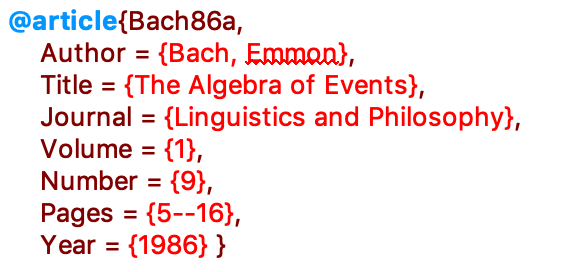
\includegraphics[scale=.5]{../../texfiles-beamer/tex-material/WissArb-latex/xelatex-bib-article}

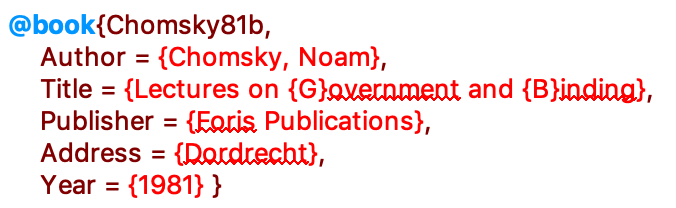
\includegraphics[scale=.5]{../../texfiles-beamer/tex-material/WissArb-latex/xelatex-bib-book}

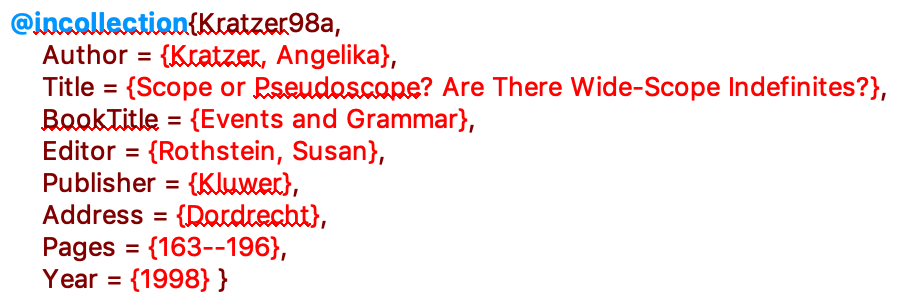
\includegraphics[scale=.5]{../../texfiles-beamer/tex-material/WissArb-latex/xelatex-bib-incollection}

\end{frame}

%%%%%%%%%%%%%%%%%%%%%%%%%%%%%%%%%%
%%%%%%%%%%%%%%%%%%%%%%%%%%%%%%%%%%
\section{Using your references}
\frame{
\frametitle{~}
\begin{multicols}{2}
\tableofcontents[currentsection,hideallsubsections]
\end{multicols}
}
%%%%%%%%%%%%%%%%%%%%%%%%%%%%%%%%%%

\begin{frame}[fragile]
\frametitle{Using your references}

Using your references is similar to using \ltxterm{ref}, but with the command \textbf{\ltxterm{cite}} (or versions of it) and the \textbf{ID} of the entry:

\begin{lstlisting}
\cite{ID}
\end{lstlisting}

%\vspace{.3cm}

If a reference should \textbf{appear in your bibliography}, but \textbf{not in your text}, then use \textbf{\ltxterm{nocite}} and the \textbf{ID}:

\begin{lstlisting}
\nocite{ID}
\end{lstlisting}

\pause 

\textbf{Example:}

\begin{lstlisting}
The following entry appear in the text and in the bibliography (cf.\ end of this 
presentation): \cite{Loebner15a}.
On the other hand, the following entry is not appearing in the text but in the 
bibliography (cf.\ end of this presentation): \nocite{ZimmermannT&Sternefeld13a}
\end{lstlisting}

\outputbox{
The following entry appear in the text and in the bibliography (cf.\ end of this 
presentation): \cite{Loebner15a}.

On the other hand, the following entry is not appearing in the text but in the 
bibliography (cf.\ end of this presentation): \nocite{ZimmermannT&Sternefeld13a}
}

\end{frame}


%%%%%%%%%%%%%%%%%%%%%%%%%%%%%%%%%%
%%%%%%%%%%%%%%%%%%%%%%%%%%%%%%%%%%
\section{Bibliography style \& bibliography}
\frame{
	\frametitle{~}
	\begin{multicols}{2}
		\tableofcontents[currentsection,hideallsubsections]
	\end{multicols}
}
%%%%%%%%%%%%%%%%%%%%%%%%%%%%%%%%%%

\begin{frame}[fragile]
\frametitle{Bibliography style \& bibliography}

\begin{itemize}
	\item The ways your \textbf{in-text citations} and your \textbf{bibliography} is formatted depends on your \textbf{bibliography style}. 
	
%	Das Aussehen des \textbf{Literaturverzeichnisses} und der im Fließtext angegebenen \textbf{Quellen} hängt vom \textbf{Bibliographiestil} ab.
	
	\item The following styles are always included (other styles are loaded for instance with packages):
	
	\begin{itemize}
		\item \ltxterm{alpha.bst}
		\item \ltxterm{abbrv.bst} (useful for abstracts)
		\item \ltxterm{plain.bst}
		\item \ltxterm{unsrt.bst}
	\end{itemize}

%	\item Die Stile sind \idR für das Englische geschrieben. Im Netz finden Sie andere Stile für das Deutsche.

\item At the position you want your bibliography to appear, put the following commands:

%Am \textbf{Ende des Dokuments} (oder an der \textbf{Position, an der die Literaturliste erscheinen soll}) wird die \textbf{Verlinkung zur eigenen Bibliographiedatenbank} erstellt. Das Literaturverzeichnis wird an dieser Stelle gedruckt.

%\item Es ist empfehlenswert den \textbf{Bibliographiestil} an der gleichen Stelle \textbf{festzulegen}.

\end{itemize}

\begin{multicols}{2}

\begin{lstlisting}
\bibliographystyle{name of style}
\bibliography{name of .bib-file} 
\end{lstlisting}

\columnbreak

\begin{lstlisting}
\bibliographystyle{langsci-unified}
\bibliography{myFirstBibliography} 
\end{lstlisting}

\end{multicols}

\end{frame}

%%%%%%%%%%%%%%%%%%%%%%%%%%%%%%%%%%
\begin{frame}[fragile]
\frametitle{Style: alpha}

\begin{figure}
\centering
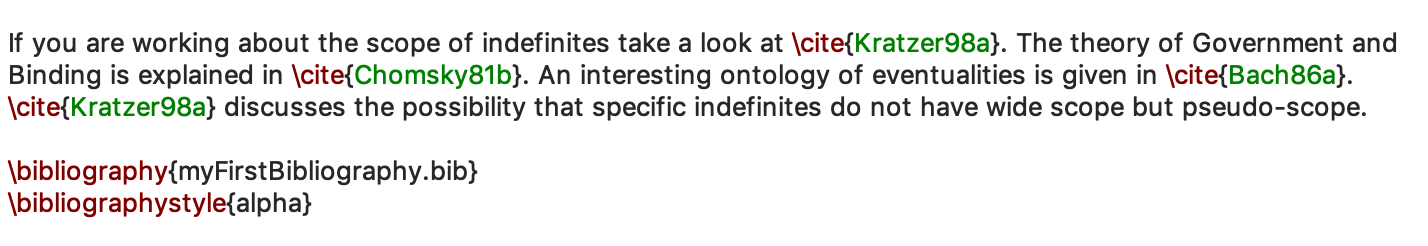
\includegraphics[width=.75\textwidth]{../../texfiles-beamer/tex-material/WissArb-latex/xelatex-bib-alpha}
\end{figure}

\begin{figure}
\centering
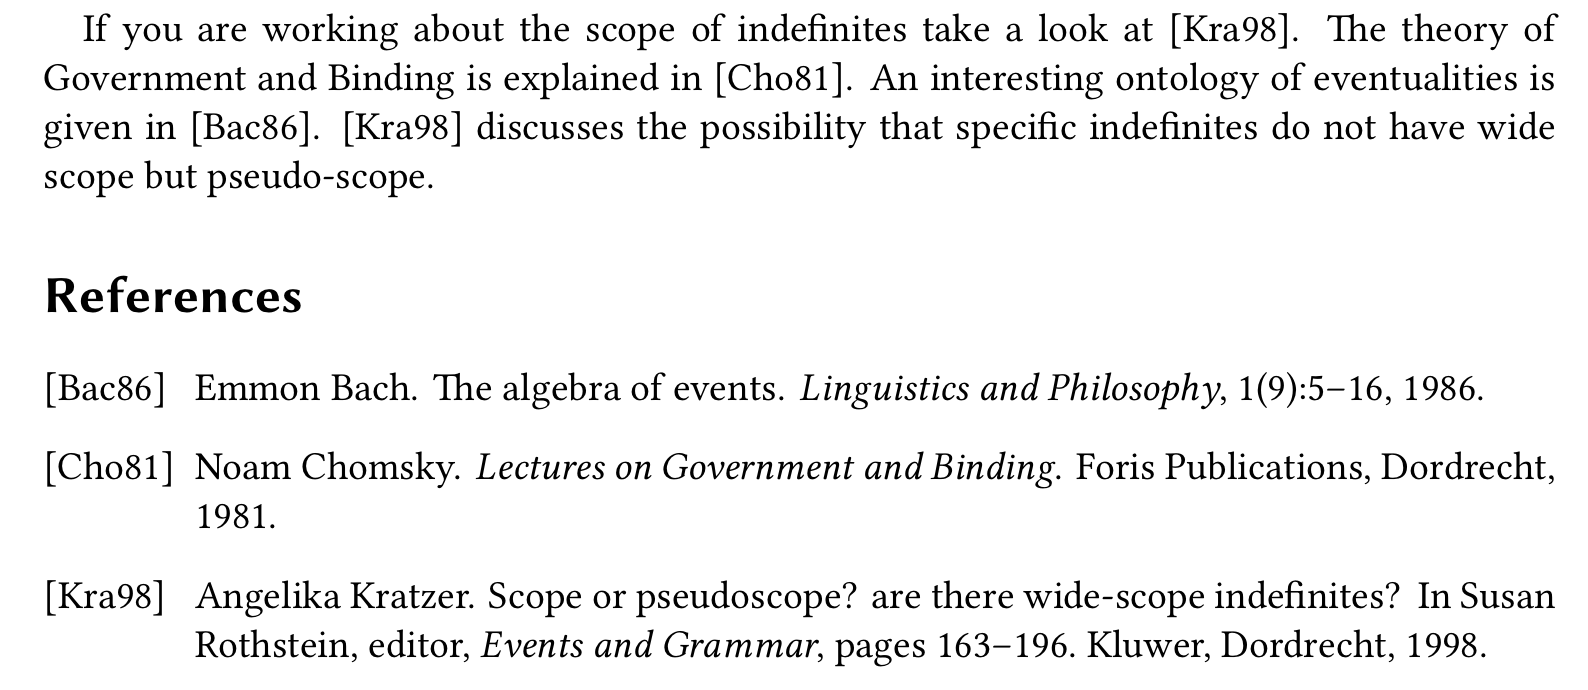
\includegraphics[width=.75\textwidth]{../../texfiles-beamer/tex-material/WissArb-latex/xelatex-bib-alpha-pdf}
\end{figure}

\end{frame}


%%%%%%%%%%%%%%%%%%%%%%%%%%%%%%%%%%
\begin{frame}[fragile]
\frametitle{Style: abbrv}

\begin{figure}
\centering
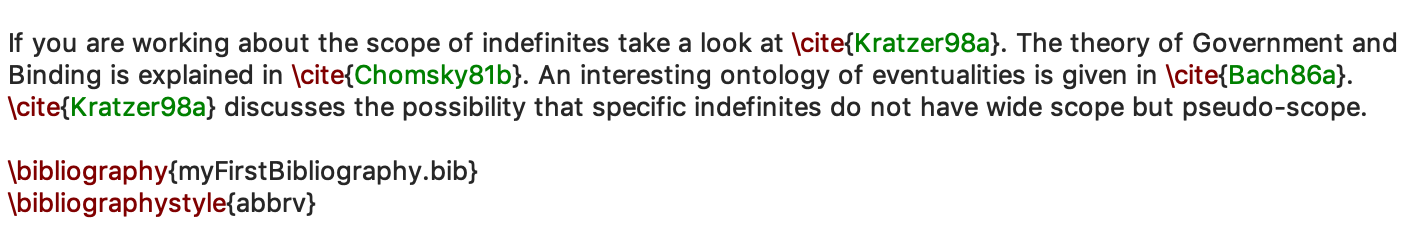
\includegraphics[width=.75\textwidth]{../../texfiles-beamer/tex-material/WissArb-latex/xelatex-bib-abbrv}
\end{figure}

\begin{figure}
\centering
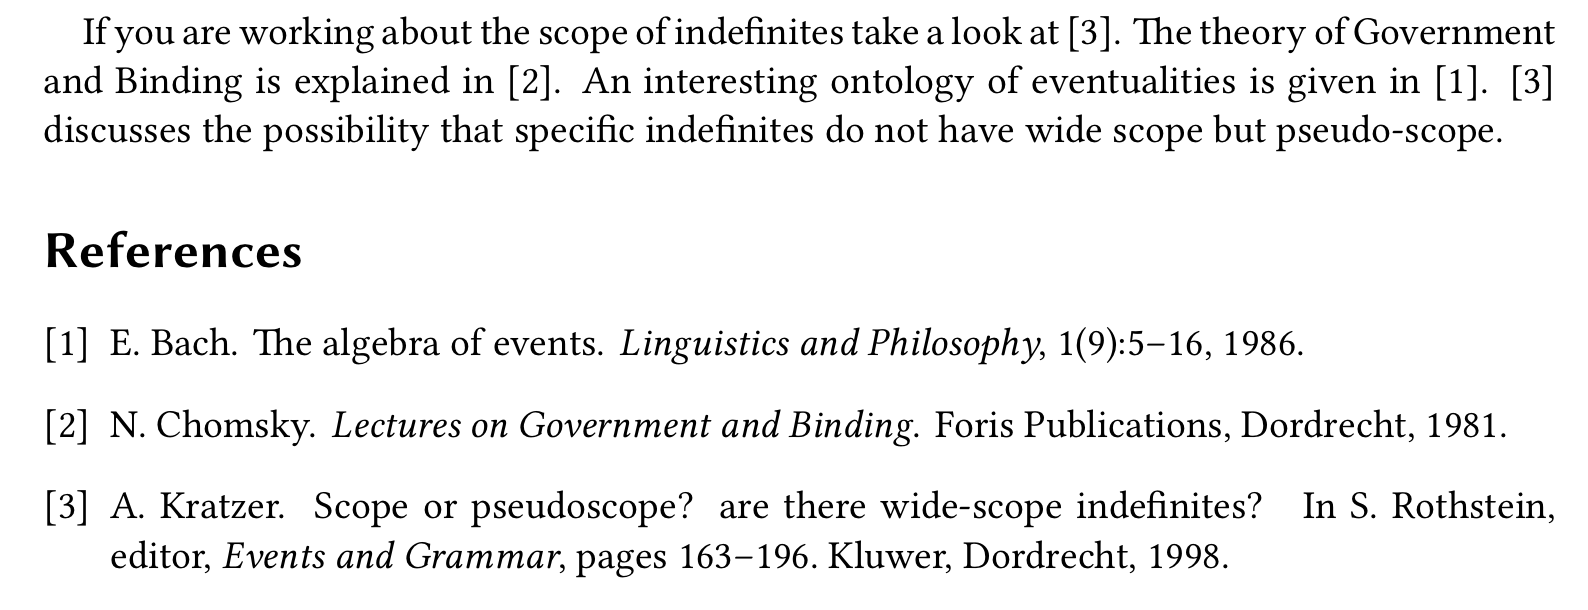
\includegraphics[width=.75\textwidth]{../../texfiles-beamer/tex-material/WissArb-latex/xelatex-bib-abbrv-pdf}
\end{figure}

\end{frame}


%%%%%%%%%%%%%%%%%%%%%%%%%%%%%%%%%%%
%\begin{frame}[fragile]
%\frametitle{Stil: plain}
%
%\begin{figure}
%\centering
%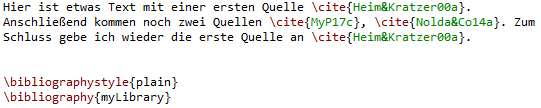
\includegraphics[width=.70\textwidth]{../../texfiles-beamer/tex-material/WissArb-latex/bib_plain_tex}
%\end{figure}
%
%\begin{figure}
%\centering
%
\includegraphics[width=.70\textwidth]{../../texfiles-beamer/tex-material/WissArb-latex/bib_plain_pdf}
%\end{figure}
%
%\end{frame}



%%%%%%%%%%%%%%%%%%%%%%%%%%%%%%%%%
\begin{frame}[fragile]
\frametitle{Exercise}


Go to \url{https://github.com/langsci/latex4linguists/blob/master/2-1.md}\\
and follow the instructions of \textbf{all blocks} in your \texttt{.tex} file.

%Download the PDF \alert{\texttt{myDocument-EX4.pdf}} and replicate it with the commands you have already learnt. Follow the instructions in the last section and install the packages.

\end{frame}


%%%%%%%%%%%%%%%%%%%%%%%%%%%%%%%%%%%
%%%%%%%%%%%%%%%%%%%%%%%%%%%%%%%%%%%
%\section{XY}
%%\frame{
%%\begin{multicols}{2}
%%\frametitle{~}
%%	\tableofcontents[currentsection]
%%\end{multicols}
%%}
%%%%%%%%%%%%%%%%%%%%%%%%%%%%%%%%%%%
%
%\begin{frame}{XY}
%
%\begin{itemize}
%	\item XY
%\end{itemize}
%
%\end{frame}


%%%%%%%%%%%%%%%%%%%%%%%%%%%%%%%%%%%%
%%%%%%%%%%%%%%%%%%%%%%%%%%%%%%%%%%%%
%\iftoggle{handout}{
%%% BEGIN handout true
%
%%%%%%%%%%%%%%%%%%%%%%%%%%%%%%%%%%%%
%	
%%Test Toggle ON
%
%}
%%% END handout true 
%%% BEGIN handout false
%{
%%%%%%%%%%%%%%%%%%%%%%%%%%%%%%%%%%%%
%
%% Test Toggle OFF
%
%}%% END handout false
%%%%%%%%%%%%%%%%%%%%%%%%%%%%%%%%%%%%